\begin{frame}{Πειραματικά αποτελέσματα: LANDFILL (sim; 5/6)}

  \begin{figure}
    \definecolor{a}{RGB}{235, 172, 35}
\definecolor{b}{RGB}{184, 0, 88}
\definecolor{c}{RGB}{0, 140, 249}
\definecolor{d}{RGB}{0, 110, 0}
\definecolor{e}{RGB}{0, 187, 173}
\definecolor{f}{RGB}{209, 99, 230}
\definecolor{g}{RGB}{178, 69, 2}

% GNUPLOT: LaTeX picture with Postscript
\begingroup
  \makeatletter
  \providecommand\color[2][]{%
    \GenericError{(gnuplot) \space\space\space\@spaces}{%
      Package color not loaded in conjunction with
      terminal option `colourtext'%
    }{See the gnuplot documentation for explanation.%
    }{Either use 'blacktext' in gnuplot or load the package
      color.sty in LaTeX.}%
    \renewcommand\color[2][]{}%
  }%
  \providecommand\includegraphics[2][]{%
    \GenericError{(gnuplot) \space\space\space\@spaces}{%
      Package graphicx or graphics not loaded%
    }{See the gnuplot documentation for explanation.%
    }{The gnuplot epslatex terminal needs graphicx.sty or graphics.sty.}%
    \renewcommand\includegraphics[2][]{}%
  }%
  \providecommand\rotatebox[2]{#2}%
  \@ifundefined{ifGPcolor}{%
    \newif\ifGPcolor
    \GPcolorfalse
  }{}%
  \@ifundefined{ifGPblacktext}{%
    \newif\ifGPblacktext
    \GPblacktexttrue
  }{}%
  % define a \g@addto@macro without @ in the name:
  \let\gplgaddtomacro\g@addto@macro
  % define empty templates for all commands taking text:
  \gdef\gplfronttext{}%
  \gdef\gplfronttext{}%
  \makeatother
  \ifGPblacktext
    % no textcolor at all
    \def\colorrgb#1{}%
    \def\colorgray#1{}%
  \else
    % gray or color?
    \ifGPcolor
      \def\colorrgb#1{\color[rgb]{#1}}%
      \def\colorgray#1{\color[gray]{#1}}%
      \expandafter\def\csname LTw\endcsname{\color{white}}%
      \expandafter\def\csname LTb\endcsname{\color{black}}%
      \expandafter\def\csname LTa\endcsname{\color{black}}%
      \expandafter\def\csname LT0\endcsname{\color[rgb]{1,0,0}}%
      \expandafter\def\csname LT1\endcsname{\color[rgb]{0,1,0}}%
      \expandafter\def\csname LT2\endcsname{\color[rgb]{0,0,1}}%
      \expandafter\def\csname LT3\endcsname{\color[rgb]{1,0,1}}%
      \expandafter\def\csname LT4\endcsname{\color[rgb]{0,1,1}}%
      \expandafter\def\csname LT5\endcsname{\color[rgb]{1,1,0}}%
      \expandafter\def\csname LT6\endcsname{\color[rgb]{0,0,0}}%
      \expandafter\def\csname LT7\endcsname{\color[rgb]{1,0.3,0}}%
      \expandafter\def\csname LT8\endcsname{\color[rgb]{0.5,0.5,0.5}}%
    \else
      % gray
      \def\colorrgb#1{\color{black}}%
      \def\colorgray#1{\color[gray]{#1}}%
      \expandafter\def\csname LTw\endcsname{\color{white}}%
      \expandafter\def\csname LTb\endcsname{\color{black}}%
      \expandafter\def\csname LTa\endcsname{\color{black}}%
      \expandafter\def\csname LT0\endcsname{\color{black}}%
      \expandafter\def\csname LT1\endcsname{\color{black}}%
      \expandafter\def\csname LT2\endcsname{\color{black}}%
      \expandafter\def\csname LT3\endcsname{\color{black}}%
      \expandafter\def\csname LT4\endcsname{\color{black}}%
      \expandafter\def\csname LT5\endcsname{\color{black}}%
      \expandafter\def\csname LT6\endcsname{\color{black}}%
      \expandafter\def\csname LT7\endcsname{\color{black}}%
      \expandafter\def\csname LT8\endcsname{\color{black}}%
    \fi
  \fi
    \setlength{\unitlength}{0.0500bp}%
    \ifx\gptboxheight\undefined%
      \newlength{\gptboxheight}%
      \newlength{\gptboxwidth}%
      \newsavebox{\gptboxtext}%
    \fi%
    \setlength{\fboxrule}{0.5pt}%
    \setlength{\fboxsep}{1pt}%
\begin{picture}(9500.00,4000.00)%
    \gplgaddtomacro\gplfronttext{%
      \colorrgb{0.15,0.15,0.15}%
      \put(1316,1730){\makebox(0,0)[r]{\strut{}0}}%
      \colorrgb{0.15,0.15,0.15}%
      \put(1316,2053){\makebox(0,0)[r]{\strut{}5}}%
      \colorrgb{0.15,0.15,0.15}%
      \put(1316,2375){\makebox(0,0)[r]{\strut{}10}}%
      \colorrgb{0.15,0.15,0.15}%
      \put(1316,2697){\makebox(0,0)[r]{\strut{}15}}%
      \colorrgb{0.15,0.15,0.15}%
      \put(1316,3019){\makebox(0,0)[r]{\strut{}20}}%
      \colorrgb{0.15,0.15,0.15}%
      \put(1316,3341){\makebox(0,0)[r]{\strut{}25}}%
      \colorrgb{0.15,0.15,0.15}%
      \put(1512,1446){\makebox(0,0){\strut{}0}}%
      \colorrgb{0.15,0.15,0.15}%
      %\put(1641,1446){\makebox(0,0){\strut{}2}}%
      \colorrgb{0.15,0.15,0.15}%
      \put(1770,1446){\makebox(0,0){\strut{}4}}%
      \colorrgb{0.15,0.15,0.15}%
      %\put(1899,1446){\makebox(0,0){\strut{}6}}%
      \colorrgb{0.15,0.15,0.15}%
      \put(2028,1446){\makebox(0,0){\strut{}8}}%
      \colorrgb{0.15,0.15,0.15}%
      %\put(2157,1446){\makebox(0,0){\strut{}10}}%
      \colorrgb{0.15,0.15,0.15}%
      \put(2286,1446){\makebox(0,0){\strut{}12}}%
    }%
    \gplgaddtomacro\gplfronttext{%
      \colorrgb{0.15,0.15,0.15}%
      \put(810,2632){\rotatebox{90}{\makebox(0,0){\strut{}$y$ [m]}}}%
      \colorrgb{0.15,0.15,0.15}%
      \put(1899,1116){\makebox(0,0){\strut{}$x$ [m]}}%
      \put(1899,300){\makebox(0,0){\strut{}$|\mathcal{H}_L| = 100$ υποθέσεις}}%
    }%
    \gplgaddtomacro\gplfronttext{%
      \colorrgb{0.15,0.15,0.15}%
      \put(3668,2933){\makebox(0,0)[r]{\strut{}\scriptsize $0\%$}}%
      \colorrgb{0.15,0.15,0.15}%
      \put(3668,3100){\makebox(0,0)[r]{\strut{}\scriptsize $25\%$}}%
      \colorrgb{0.15,0.15,0.15}%
      \put(3668,3266){\makebox(0,0)[r]{\strut{}\scriptsize $50\%$}}%
      \colorrgb{0.15,0.15,0.15}%
      \put(3668,3433){\makebox(0,0)[r]{\strut{}\scriptsize $75\%$}}%
      \colorrgb{0.15,0.15,0.15}%
      \put(3668,3599){\makebox(0,0)[r]{\strut{}\scriptsize $100\%$}}%
      \colorrgb{0.15,0.15,0.15}%
      \put(3936,2813){\makebox(0,0){\strut{}\scriptsize \textcolor{a}{$\bm{p}_a^L$}}}%
      \colorrgb{0.15,0.15,0.15}%
      \put(4207,2813){\makebox(0,0){\strut{}\scriptsize \textcolor{b}{$\bm{p}_b^L$}}}%
      \colorrgb{0.15,0.15,0.15}%
      \put(4478,2813){\makebox(0,0){\strut{}\scriptsize \textcolor{c}{$\bm{p}_c^L$}}}%
      \colorrgb{0.15,0.15,0.15}%
      \put(4750,2813){\makebox(0,0){\strut{}\scriptsize \textcolor{d}{$\bm{p}_d^L$}}}%
      \colorrgb{0.15,0.15,0.15}%
      \put(5021,2813){\makebox(0,0){\strut{}\scriptsize \textcolor{e}{$\bm{p}_e^L$}}}%
      \colorrgb{0.15,0.15,0.15}%
      \put(5292,2813){\makebox(0,0){\strut{}\scriptsize \textcolor{f}{$\bm{p}_f^L$}}}%
      \colorrgb{0.15,0.15,0.15}%
      \put(5563,2813){\makebox(0,0){\strut{}\scriptsize \textcolor{g}{$\bm{p}_g^L$}}}%
    }%
    \gplgaddtomacro\gplfronttext{%
      \colorrgb{0.00,0.00,0.00}%
      \put(6000,3819){\makebox(0,0){\strut{}\footnotesize Ποσοστά αποτυχιών}}%
    }%
    \gplgaddtomacro\gplfronttext{%
      \colorrgb{0.15,0.15,0.15}%
      \put(6518,2933){\makebox(0,0)[r]{\strut{}\scriptsize $0\%$}}%
      \colorrgb{0.15,0.15,0.15}%
      \put(6518,3100){\makebox(0,0)[r]{\strut{}\scriptsize $25\%$}}%
      \colorrgb{0.15,0.15,0.15}%
      \put(6518,3266){\makebox(0,0)[r]{\strut{}\scriptsize $50\%$}}%
      \colorrgb{0.15,0.15,0.15}%
      \put(6518,3433){\makebox(0,0)[r]{\strut{}\scriptsize $75\%$}}%
      \colorrgb{0.15,0.15,0.15}%
      \put(6518,3599){\makebox(0,0)[r]{\strut{}\scriptsize $100\%$}}%
      \colorrgb{0.15,0.15,0.15}%
      \put(6786,2813){\makebox(0,0){\strut{}\scriptsize \textcolor{a}{$\bm{p}_a^L$}}}%
      \colorrgb{0.15,0.15,0.15}%
      \put(7057,2813){\makebox(0,0){\strut{}\scriptsize \textcolor{b}{$\bm{p}_b^L$}}}%
      \colorrgb{0.15,0.15,0.15}%
      \put(7328,2813){\makebox(0,0){\strut{}\scriptsize \textcolor{c}{$\bm{p}_c^L$}}}%
      \colorrgb{0.15,0.15,0.15}%
      \put(7600,2813){\makebox(0,0){\strut{}\scriptsize \textcolor{d}{$\bm{p}_d^L$}}}%
      \colorrgb{0.15,0.15,0.15}%
      \put(7871,2813){\makebox(0,0){\strut{}\scriptsize \textcolor{e}{$\bm{p}_e^L$}}}%
      \colorrgb{0.15,0.15,0.15}%
      \put(8142,2813){\makebox(0,0){\strut{}\scriptsize \textcolor{f}{$\bm{p}_f^L$}}}%
      \colorrgb{0.15,0.15,0.15}%
      \put(8413,2813){\makebox(0,0){\strut{}\scriptsize \textcolor{g}{$\bm{p}_g^L$}}}%
    }%
    \gplgaddtomacro\gplfronttext{%
    }%
    \gplgaddtomacro\gplfronttext{%
      \colorrgb{0.15,0.15,0.15}%
      \put(3668,1666){\makebox(0,0)[r]{\strut{}\scriptsize $0.25$}}%
      \colorrgb{0.15,0.15,0.15}%
      \put(3668,1833){\makebox(0,0)[r]{\strut{}\scriptsize $0.30$}}%
      \colorrgb{0.15,0.15,0.15}%
      \put(3668,1999){\makebox(0,0)[r]{\strut{}\scriptsize $0.35$}}%
      \colorrgb{0.15,0.15,0.15}%
      \put(3668,2166){\makebox(0,0)[r]{\strut{}\scriptsize $0.40$}}%
      \colorrgb{0.15,0.15,0.15}%
      \put(3668,2332){\makebox(0,0)[r]{\strut{}\scriptsize $0.45$}}%
      \colorrgb{0.15,0.15,0.15}%
      \put(3717,1546){\makebox(0,0){\strut{}\scriptsize $\sigma_R$:}}%
      \put(4117,1546){\makebox(0,0){\strut{}\scriptsize $0.01$}}%
      \colorrgb{0.15,0.15,0.15}%
      \put(4750,1546){\makebox(0,0){\strut{}\scriptsize $0.02$}}%
      \colorrgb{0.15,0.15,0.15}%
      \put(5383,1546){\makebox(0,0){\strut{}\scriptsize $0.05$}}%
    }%
    \gplgaddtomacro\gplfronttext{%
      \colorrgb{0.00,0.00,0.00}%
      \put(6000,2552){\makebox(0,0){\strut{}\footnotesize Μέσο σφάλμα στάσης [$(\text{m}^2 + \text{rad}^2)^{1/2}$]}}%
    }%
    \gplgaddtomacro\gplfronttext{%
      \colorrgb{0.15,0.15,0.15}%
      \put(6518,1666){\makebox(0,0)[r]{\strut{}\scriptsize $0.25$}}%
      \colorrgb{0.15,0.15,0.15}%
      \put(6518,1833){\makebox(0,0)[r]{\strut{}\scriptsize $0.30$}}%
      \colorrgb{0.15,0.15,0.15}%
      \put(6518,1999){\makebox(0,0)[r]{\strut{}\scriptsize $0.35$}}%
      \colorrgb{0.15,0.15,0.15}%
      \put(6518,2166){\makebox(0,0)[r]{\strut{}\scriptsize $0.40$}}%
      \colorrgb{0.15,0.15,0.15}%
      \put(6518,2332){\makebox(0,0)[r]{\strut{}\scriptsize $0.45$}}%
      \colorrgb{0.15,0.15,0.15}%
      \put(6567,1546){\makebox(0,0){\strut{}\scriptsize $\sigma_R$:}}%
      \put(6967,1546){\makebox(0,0){\strut{}\scriptsize $0.01$}}%
      \colorrgb{0.15,0.15,0.15}%
      \put(7600,1546){\makebox(0,0){\strut{}\scriptsize $0.02$}}%
      \colorrgb{0.15,0.15,0.15}%
      \put(8233,1546){\makebox(0,0){\strut{}\scriptsize $0.05$}}%
    }%
    \gplgaddtomacro\gplfronttext{%
    }%
    \gplgaddtomacro\gplfronttext{%
      \colorrgb{0.15,0.15,0.15}%
      \put(3668,400){\makebox(0,0)[r]{\strut{}\scriptsize $200$}}%
      \colorrgb{0.15,0.15,0.15}%
      \put(3668,622){\makebox(0,0)[r]{\strut{}\scriptsize $250$}}%
      \colorrgb{0.15,0.15,0.15}%
      \put(3668,844){\makebox(0,0)[r]{\strut{}\scriptsize $300$}}%
      \colorrgb{0.15,0.15,0.15}%
      \put(3668,1066){\makebox(0,0)[r]{\strut{}\scriptsize $350$}}%
      \colorrgb{0.15,0.15,0.15}%
      \put(3717,280){\makebox(0,0){\strut{}\scriptsize $\sigma_R$:}}%
      \put(4117,280){\makebox(0,0){\strut{}\scriptsize $0.01$}}%
      \colorrgb{1.15,0.15,0.15}%
      \put(4750,280){\makebox(0,0){\strut{}\scriptsize $0.02$}}%
      \colorrgb{1.15,0.15,0.15}%
      \put(5383,280){\makebox(0,0){\strut{}\scriptsize $0.05$}}%
    }%
    \gplgaddtomacro\gplfronttext{%
      \colorrgb{0.00,0.00,0.00}%
      \put(6000,1286){\makebox(0,0){\strut{}\footnotesize Μέσος χρόνος εκτέλεσης ανά υπόθεση [ms]}}%
    }%
    \gplgaddtomacro\gplfronttext{%
      \colorrgb{0.15,0.15,0.15}%
      \put(6518,400){\makebox(0,0)[r]{\strut{}\scriptsize $200$}}%
      \colorrgb{0.15,0.15,0.15}%
      \put(6518,622){\makebox(0,0)[r]{\strut{}\scriptsize $250$}}%
      \colorrgb{0.15,0.15,0.15}%
      \put(6518,844){\makebox(0,0)[r]{\strut{}\scriptsize $300$}}%
      \colorrgb{0.15,0.15,0.15}%
      \put(6518,1066){\makebox(0,0)[r]{\strut{}\scriptsize $350$}}%
      \colorrgb{0.00,0.00,0.00}%
      \put(6567,280){\makebox(0,0){\strut{}\scriptsize $\sigma_R$:}}%
      \put(6967,280){\makebox(0,0){\strut{}\scriptsize $0.01$}}%
      \colorrgb{0.00,0.00,0.00}%
      \put(7600,280){\makebox(0,0){\strut{}\scriptsize $0.02$}}%
      \colorrgb{0.00,0.00,0.00}%
      \put(8233,280){\makebox(0,0){\strut{}\scriptsize $0.05$}}%
    }%
    \gplgaddtomacro\gplfronttext{%
    }%
    \put(0,0){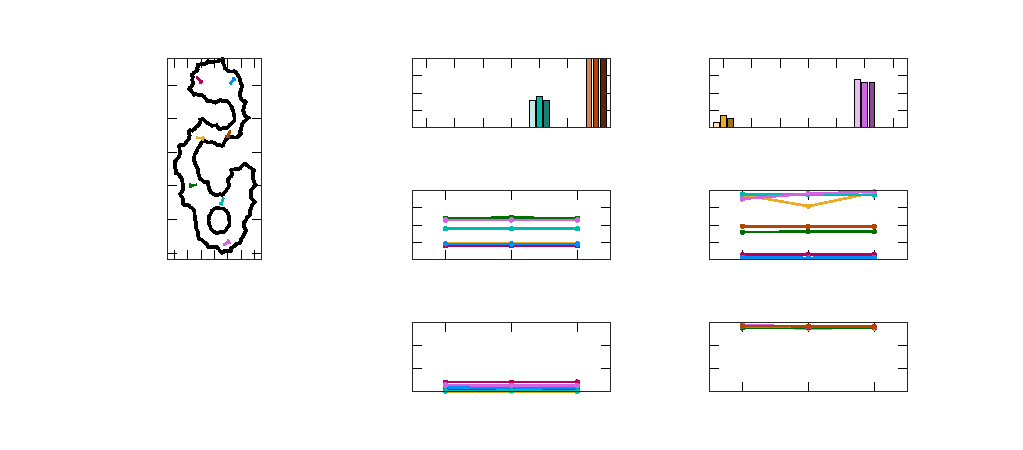
\includegraphics{./figures/slides/ch5/experiments//results_landfill}}%
    \gplfronttext
  \end{picture}%
\endgroup

  \end{figure}


\note{\footnotesize

Το περιβάλλον LANDFILL το φτιάξαμε από το μηδέν ως ένα περιβάλλον που δεν
περιλαμβάνει ευθείες γραμμές, ή γωνίες, ώστε να δείξουμε πως σε αντίθεση με μία
κλάση μεθόδων της βιβλιογραφίας, η μέθοδος που οικοδομήσαμε είναι αναλλοίωτη
των περιβαλλόντων και δεν απαιτεί να εμφανίζουν συγκεκριμένα features,}
\end{frame}
